\documentclass[1p]{elsarticle_modified}
%\bibliographystyle{elsarticle-num}

%\usepackage[colorlinks]{hyperref}
%\usepackage{abbrmath_seonhwa} %\Abb, \Ascr, \Acal ,\Abf, \Afrak
\usepackage{amsfonts}
\usepackage{amssymb}
\usepackage{amsmath}
\usepackage{amsthm}
\usepackage{scalefnt}
\usepackage{amsbsy}
\usepackage{kotex}
\usepackage{caption}
\usepackage{subfig}
\usepackage{color}
\usepackage{graphicx}
\usepackage{xcolor} %% white, black, red, green, blue, cyan, magenta, yellow
\usepackage{float}
\usepackage{setspace}
\usepackage{hyperref}

\usepackage{tikz}
\usetikzlibrary{arrows}

\usepackage{multirow}
\usepackage{array} % fixed length table
\usepackage{hhline}

%%%%%%%%%%%%%%%%%%%%%
\makeatletter
\renewcommand*\env@matrix[1][\arraystretch]{%
	\edef\arraystretch{#1}%
	\hskip -\arraycolsep
	\let\@ifnextchar\new@ifnextchar
	\array{*\c@MaxMatrixCols c}}
\makeatother %https://tex.stackexchange.com/questions/14071/how-can-i-increase-the-line-spacing-in-a-matrix
%%%%%%%%%%%%%%%

\usepackage[normalem]{ulem}

\newcommand{\msout}[1]{\ifmmode\text{\sout{\ensuremath{#1}}}\else\sout{#1}\fi}
%SOURCE: \msout is \stkout macro in https://tex.stackexchange.com/questions/20609/strikeout-in-math-mode

\newcommand{\cancel}[1]{
	\ifmmode
	{\color{red}\msout{#1}}
	\else
	{\color{red}\sout{#1}}
	\fi
}

\newcommand{\add}[1]{
	{\color{blue}\uwave{#1}}
}

\newcommand{\replace}[2]{
	\ifmmode
	{\color{red}\msout{#1}}{\color{blue}\uwave{#2}}
	\else
	{\color{red}\sout{#1}}{\color{blue}\uwave{#2}}
	\fi
}

\newcommand{\Sol}{\mathcal{S}} %segment
\newcommand{\D}{D} %diagram
\newcommand{\A}{\mathcal{A}} %arc


%%%%%%%%%%%%%%%%%%%%%%%%%%%%%5 test

\def\sl{\operatorname{\textup{SL}}(2,\Cbb)}
\def\psl{\operatorname{\textup{PSL}}(2,\Cbb)}
\def\quan{\mkern 1mu \triangleright \mkern 1mu}

\theoremstyle{definition}
\newtheorem{thm}{Theorem}[section]
\newtheorem{prop}[thm]{Proposition}
\newtheorem{lem}[thm]{Lemma}
\newtheorem{ques}[thm]{Question}
\newtheorem{cor}[thm]{Corollary}
\newtheorem{defn}[thm]{Definition}
\newtheorem{exam}[thm]{Example}
\newtheorem{rmk}[thm]{Remark}
\newtheorem{alg}[thm]{Algorithm}

\newcommand{\I}{\sqrt{-1}}
\begin{document}

%\begin{frontmatter}
%
%\title{Boundary parabolic representations of knots up to 8 crossings}
%
%%% Group authors per affiliation:
%\author{Yunhi Cho} 
%\address{Department of Mathematics, University of Seoul, Seoul, Korea}
%\ead{yhcho@uos.ac.kr}
%
%
%\author{Seonhwa Kim} %\fnref{s_kim}}
%\address{Center for Geometry and Physics, Institute for Basic Science, Pohang, 37673, Korea}
%\ead{ryeona17@ibs.re.kr}
%
%\author{Hyuk Kim}
%\address{Department of Mathematical Sciences, Seoul National University, Seoul 08826, Korea}
%\ead{hyukkim@snu.ac.kr}
%
%\author{Seokbeom Yoon}
%\address{Department of Mathematical Sciences, Seoul National University, Seoul, 08826,  Korea}
%\ead{sbyoon15@snu.ac.kr}
%
%\begin{abstract}
%We find all boundary parabolic representation of knots up to 8 crossings.
%
%\end{abstract}
%\begin{keyword}
%    \MSC[2010] 57M25 
%\end{keyword}
%
%\end{frontmatter}

%\linenumbers
%\tableofcontents
%
\newcommand\colored[1]{\textcolor{white}{\rule[-0.35ex]{0.8em}{1.4ex}}\kern-0.8em\color{red} #1}%
%\newcommand\colored[1]{\textcolor{white}{ #1}\kern-2.17ex	\textcolor{white}{ #1}\kern-1.81ex	\textcolor{white}{ #1}\kern-2.15ex\color{red}#1	}

{\Large $\underline{12n_{0447}~(K12n_{0447})}$}

\setlength{\tabcolsep}{10pt}
\renewcommand{\arraystretch}{1.6}
\vspace{1cm}\begin{tabular}{m{100pt}>{\centering\arraybackslash}m{274pt}}
\multirow{5}{120pt}{
	\centering
	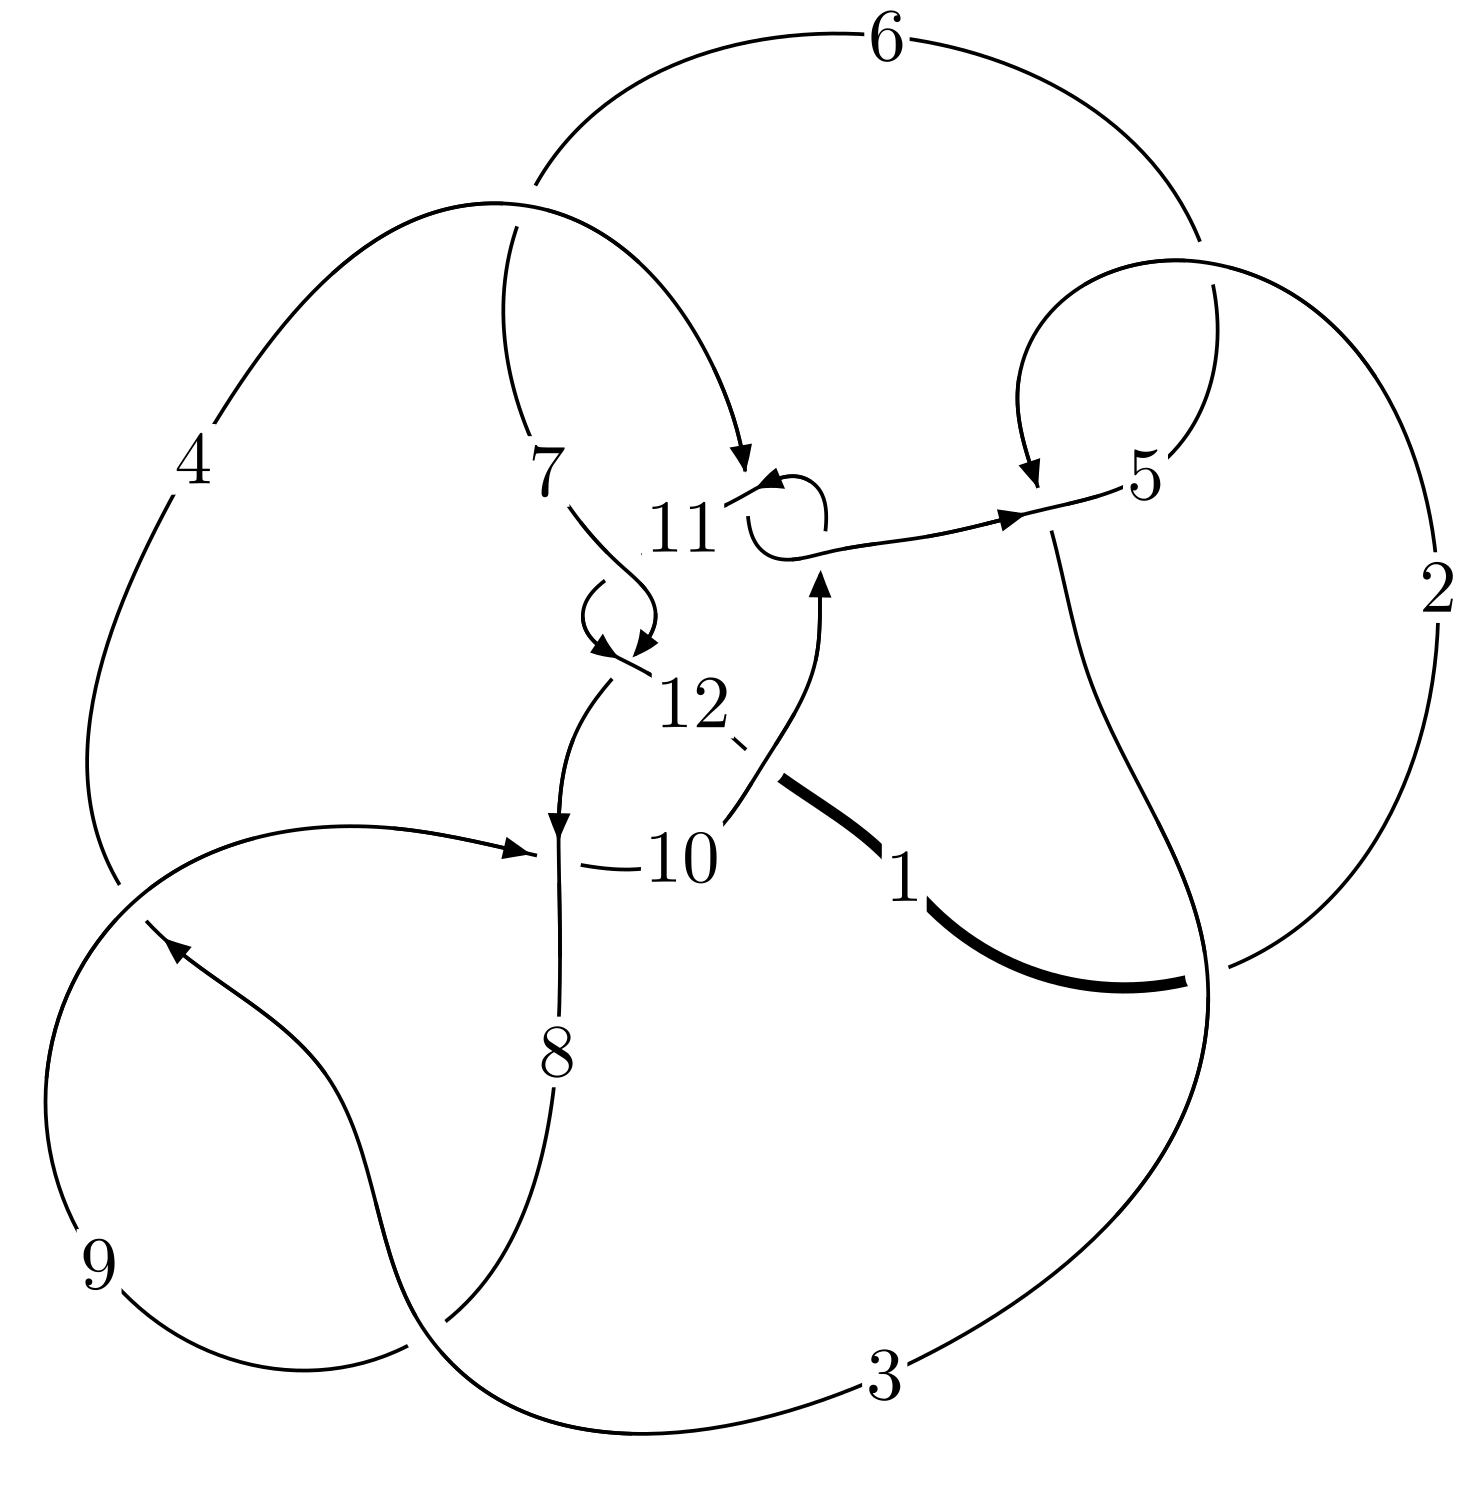
\includegraphics[width=112pt]{../../../GIT/diagram.site/Diagrams/png/2536_12n_0447.png}\\
\ \ \ A knot diagram\footnotemark}&
\allowdisplaybreaks
\textbf{Linearized knot diagam} \\
\cline{2-2}
 &
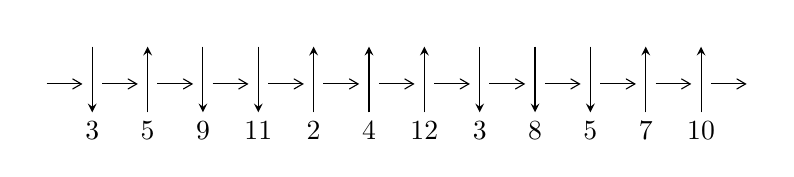
\begin{tikzpicture}[x=20pt, y=17pt]
	% nodes
	\node (C0) at (0, 0) {};
	\node (C1) at (1, 0) {};
	\node (C1U) at (1, +1) {};
	\node (C1D) at (1, -1) {3};

	\node (C2) at (2, 0) {};
	\node (C2U) at (2, +1) {};
	\node (C2D) at (2, -1) {5};

	\node (C3) at (3, 0) {};
	\node (C3U) at (3, +1) {};
	\node (C3D) at (3, -1) {9};

	\node (C4) at (4, 0) {};
	\node (C4U) at (4, +1) {};
	\node (C4D) at (4, -1) {11};

	\node (C5) at (5, 0) {};
	\node (C5U) at (5, +1) {};
	\node (C5D) at (5, -1) {2};

	\node (C6) at (6, 0) {};
	\node (C6U) at (6, +1) {};
	\node (C6D) at (6, -1) {4};

	\node (C7) at (7, 0) {};
	\node (C7U) at (7, +1) {};
	\node (C7D) at (7, -1) {12};

	\node (C8) at (8, 0) {};
	\node (C8U) at (8, +1) {};
	\node (C8D) at (8, -1) {3};

	\node (C9) at (9, 0) {};
	\node (C9U) at (9, +1) {};
	\node (C9D) at (9, -1) {8};

	\node (C10) at (10, 0) {};
	\node (C10U) at (10, +1) {};
	\node (C10D) at (10, -1) {5};

	\node (C11) at (11, 0) {};
	\node (C11U) at (11, +1) {};
	\node (C11D) at (11, -1) {7};

	\node (C12) at (12, 0) {};
	\node (C12U) at (12, +1) {};
	\node (C12D) at (12, -1) {10};
	\node (C13) at (13, 0) {};

	% arrows
	\draw[->,>={angle 60}]
	(C0) edge (C1) (C1) edge (C2) (C2) edge (C3) (C3) edge (C4) (C4) edge (C5) (C5) edge (C6) (C6) edge (C7) (C7) edge (C8) (C8) edge (C9) (C9) edge (C10) (C10) edge (C11) (C11) edge (C12) (C12) edge (C13) ;	\draw[->,>=stealth]
	(C1U) edge (C1D) (C2D) edge (C2U) (C3U) edge (C3D) (C4U) edge (C4D) (C5D) edge (C5U) (C6D) edge (C6U) (C7D) edge (C7U) (C8U) edge (C8D) (C9U) edge (C9D) (C10U) edge (C10D) (C11D) edge (C11U) (C12D) edge (C12U) ;
	\end{tikzpicture} \\
\hhline{~~} \\& 
\textbf{Solving Sequence} \\ \cline{2-2} 
 &
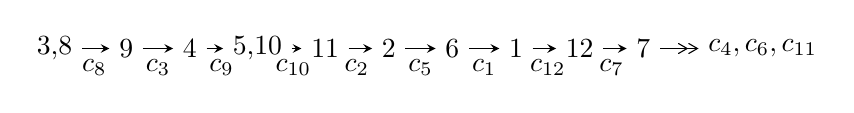
\begin{tikzpicture}[x=23pt, y=7pt]
	% node
	\node (A0) at (-1/8, 0) {3,8};
	\node (A1) at (1, 0) {9};
	\node (A2) at (2, 0) {4};
	\node (A3) at (49/16, 0) {5,10};
	\node (A4) at (33/8, 0) {11};
	\node (A5) at (41/8, 0) {2};
	\node (A6) at (49/8, 0) {6};
	\node (A7) at (57/8, 0) {1};
	\node (A8) at (65/8, 0) {12};
	\node (A9) at (73/8, 0) {7};
	\node (C1) at (1/2, -1) {$c_{8}$};
	\node (C2) at (3/2, -1) {$c_{3}$};
	\node (C3) at (5/2, -1) {$c_{9}$};
	\node (C4) at (29/8, -1) {$c_{10}$};
	\node (C5) at (37/8, -1) {$c_{2}$};
	\node (C6) at (45/8, -1) {$c_{5}$};
	\node (C7) at (53/8, -1) {$c_{1}$};
	\node (C8) at (61/8, -1) {$c_{12}$};
	\node (C9) at (69/8, -1) {$c_{7}$};
	\node (A10) at (11, 0) {$c_{4},c_{6},c_{11}$};

	% edge
	\draw[->,>=stealth]	
	(A0) edge (A1) (A1) edge (A2) (A2) edge (A3) (A3) edge (A4) (A4) edge (A5) (A5) edge (A6) (A6) edge (A7) (A7) edge (A8) (A8) edge (A9) ;
	\draw[->>,>={angle 60}]	
	(A9) edge (A10);
\end{tikzpicture} \\ 

\end{tabular} \\

\footnotetext{
The image of knot diagram is generated by the software ``\textbf{Draw programme}" developed by Andrew Bartholomew(\url{http://www.layer8.co.uk/maths/draw/index.htm\#Running-draw}), where we modified some parts for our purpose(\url{https://github.com/CATsTAILs/LinksPainter}).
}\phantom \\ \newline 
\centering \textbf{Ideals for irreducible components\footnotemark of $X_{\text{par}}$} 
 
\begin{align*}
I^u_{1}&=\langle 
-2.24038\times10^{33} u^{47}-1.35892\times10^{32} u^{46}+\cdots+2.30349\times10^{33} b+1.34156\times10^{34},\\
\phantom{I^u_{1}}&\phantom{= \langle  }1.73741\times10^{34} u^{47}-3.00948\times10^{33} u^{46}+\cdots+1.15175\times10^{34} a-1.11706\times10^{35},\;u^{48}- u^{47}+\cdots-2 u+5\rangle \\
I^u_{2}&=\langle 
- u^2 a+u^3+b+a- u,\;a^2 u^2+a^3+1,\;u^4- u^2+1\rangle \\
\\
\end{align*}
\raggedright * 2 irreducible components of $\dim_{\mathbb{C}}=0$, with total 60 representations.\\
\footnotetext{All coefficients of polynomials are rational numbers. But the coefficients are sometimes approximated in decimal forms when there is not enough margin.}
\newpage
\renewcommand{\arraystretch}{1}
\centering \section*{I. $I^u_{1}= \langle -2.24\times10^{33} u^{47}-1.36\times10^{32} u^{46}+\cdots+2.30\times10^{33} b+1.34\times10^{34},\;1.74\times10^{34} u^{47}-3.01\times10^{33} u^{46}+\cdots+1.15\times10^{34} a-1.12\times10^{35},\;u^{48}- u^{47}+\cdots-2 u+5 \rangle$}
\flushleft \textbf{(i) Arc colorings}\\
\begin{tabular}{m{7pt} m{180pt} m{7pt} m{180pt} }
\flushright $a_{3}=$&$\begin{pmatrix}0\\u\end{pmatrix}$ \\
\flushright $a_{8}=$&$\begin{pmatrix}1\\0\end{pmatrix}$ \\
\flushright $a_{9}=$&$\begin{pmatrix}1\\u^2\end{pmatrix}$ \\
\flushright $a_{4}=$&$\begin{pmatrix}- u\\- u^3+u\end{pmatrix}$ \\
\flushright $a_{5}=$&$\begin{pmatrix}-1.50850 u^{47}+0.261297 u^{46}+\cdots+4.48572 u+9.69889\\0.972603 u^{47}+0.0589938 u^{46}+\cdots-0.659198 u-5.82402\end{pmatrix}$ \\
\flushright $a_{10}=$&$\begin{pmatrix}- u^2+1\\u^2\end{pmatrix}$ \\
\flushright $a_{11}=$&$\begin{pmatrix}1.16480 u^{47}-0.192201 u^{46}+\cdots-4.27812 u-2.98881\\1.24721 u^{47}-0.462790 u^{46}+\cdots-6.68188 u-7.54251\end{pmatrix}$ \\
\flushright $a_{2}=$&$\begin{pmatrix}1.76087 u^{47}+0.00355222 u^{46}+\cdots-4.42873 u-9.58615\\0.817561 u^{47}-0.0937876 u^{46}+\cdots-5.25658 u-6.61698\end{pmatrix}$ \\
\flushright $a_{6}=$&$\begin{pmatrix}-1.61232 u^{47}+0.251322 u^{46}+\cdots+3.62117 u+8.11692\\-0.821845 u^{47}+0.0692617 u^{46}+\cdots+6.06620 u+5.24702\end{pmatrix}$ \\
\flushright $a_{1}=$&$\begin{pmatrix}1.76087 u^{47}+0.00355222 u^{46}+\cdots-4.42873 u-9.58615\\-0.673929 u^{47}-0.140698 u^{46}+\cdots+0.0189389 u+2.20515\end{pmatrix}$ \\
\flushright $a_{12}=$&$\begin{pmatrix}1.78030 u^{47}+0.0974277 u^{46}+\cdots-4.61437 u-9.37957\\0.553189 u^{47}-0.0489697 u^{46}+\cdots-3.34948 u-4.95558\end{pmatrix}$ \\
\flushright $a_{7}=$&$\begin{pmatrix}-2.55276 u^{47}+0.387556 u^{46}+\cdots+8.31343 u+13.4329\\-0.486776 u^{47}+0.132833 u^{46}+\cdots+4.46775 u+3.95207\end{pmatrix}$\\&\end{tabular}
\flushleft \textbf{(ii) Obstruction class $= -1$}\\~\\
\flushleft \textbf{(iii) Cusp Shapes $= -0.327963 u^{47}-0.0729656 u^{46}+\cdots-4.23858 u-0.466106$}\\~\\
\newpage\renewcommand{\arraystretch}{1}
\flushleft \textbf{(iv) u-Polynomials at the component}\newline \\
\begin{tabular}{m{50pt}|m{274pt}}
Crossings & \hspace{64pt}u-Polynomials at each crossing \\
\hline $$\begin{aligned}c_{1}\end{aligned}$$&$\begin{aligned}
&u^{48}+53 u^{47}+\cdots-27678 u+289
\end{aligned}$\\
\hline $$\begin{aligned}c_{2},c_{5}\end{aligned}$$&$\begin{aligned}
&u^{48}+3 u^{47}+\cdots-142 u+17
\end{aligned}$\\
\hline $$\begin{aligned}c_{3},c_{8}\end{aligned}$$&$\begin{aligned}
&u^{48}- u^{47}+\cdots-2 u+5
\end{aligned}$\\
\hline $$\begin{aligned}c_{4},c_{10}\end{aligned}$$&$\begin{aligned}
&u^{48}- u^{47}+\cdots-8 u+1
\end{aligned}$\\
\hline $$\begin{aligned}c_{6}\end{aligned}$$&$\begin{aligned}
&u^{48}+5 u^{47}+\cdots-7742 u+26561
\end{aligned}$\\
\hline $$\begin{aligned}c_{7},c_{11}\end{aligned}$$&$\begin{aligned}
&u^{48}- u^{47}+\cdots-14 u+1
\end{aligned}$\\
\hline $$\begin{aligned}c_{9}\end{aligned}$$&$\begin{aligned}
&u^{48}+29 u^{47}+\cdots-36 u+25
\end{aligned}$\\
\hline $$\begin{aligned}c_{12}\end{aligned}$$&$\begin{aligned}
&u^{48}+3 u^{47}+\cdots+4284478 u+1826857
\end{aligned}$\\
\hline
\end{tabular}\\~\\
\newpage\renewcommand{\arraystretch}{1}
\flushleft \textbf{(v) Riley Polynomials at the component}\newline \\
\begin{tabular}{m{50pt}|m{274pt}}
Crossings & \hspace{64pt}Riley Polynomials at each crossing \\
\hline $$\begin{aligned}c_{1}\end{aligned}$$&$\begin{aligned}
&y^{48}-111 y^{47}+\cdots-298879486 y+83521
\end{aligned}$\\
\hline $$\begin{aligned}c_{2},c_{5}\end{aligned}$$&$\begin{aligned}
&y^{48}+53 y^{47}+\cdots-27678 y+289
\end{aligned}$\\
\hline $$\begin{aligned}c_{3},c_{8}\end{aligned}$$&$\begin{aligned}
&y^{48}-29 y^{47}+\cdots+36 y+25
\end{aligned}$\\
\hline $$\begin{aligned}c_{4},c_{10}\end{aligned}$$&$\begin{aligned}
&y^{48}+13 y^{47}+\cdots+14 y+1
\end{aligned}$\\
\hline $$\begin{aligned}c_{6}\end{aligned}$$&$\begin{aligned}
&y^{48}+31 y^{47}+\cdots+12208109238 y+705486721
\end{aligned}$\\
\hline $$\begin{aligned}c_{7},c_{11}\end{aligned}$$&$\begin{aligned}
&y^{48}-39 y^{47}+\cdots-86 y+1
\end{aligned}$\\
\hline $$\begin{aligned}c_{9}\end{aligned}$$&$\begin{aligned}
&y^{48}-13 y^{47}+\cdots-28896 y+625
\end{aligned}$\\
\hline $$\begin{aligned}c_{12}\end{aligned}$$&$\begin{aligned}
&y^{48}+41 y^{47}+\cdots+44880385612764 y+3337406498449
\end{aligned}$\\
\hline
\end{tabular}\\~\\
\newpage\flushleft \textbf{(vi) Complex Volumes and Cusp Shapes}
$$\begin{array}{c|c|c}  
\text{Solutions to }I^u_{1}& \I (\text{vol} + \sqrt{-1}CS) & \text{Cusp shape}\\
 \hline 
\begin{aligned}
u &= -0.108352 + 0.991513 I \\
a &= -1.65182 - 0.00446 I \\
b &= \phantom{-}1.36066 + 0.53287 I\end{aligned}
 & -7.23468 - 3.54967 I & -1.53238 + 2.33493 I \\ \hline\begin{aligned}
u &= -0.108352 - 0.991513 I \\
a &= -1.65182 + 0.00446 I \\
b &= \phantom{-}1.36066 - 0.53287 I\end{aligned}
 & -7.23468 + 3.54967 I & -1.53238 - 2.33493 I \\ \hline\begin{aligned}
u &= \phantom{-}0.174873 + 0.981711 I \\
a &= \phantom{-}1.74425 + 0.00932 I \\
b &= -1.41834 + 0.60453 I\end{aligned}
 & -2.92990 + 8.29102 I & \phantom{-}2.36664 - 4.88040 I \\ \hline\begin{aligned}
u &= \phantom{-}0.174873 - 0.981711 I \\
a &= \phantom{-}1.74425 - 0.00932 I \\
b &= -1.41834 - 0.60453 I\end{aligned}
 & -2.92990 - 8.29102 I & \phantom{-}2.36664 + 4.88040 I \\ \hline\begin{aligned}
u &= \phantom{-}0.030174 + 0.983574 I \\
a &= \phantom{-}1.55380 - 0.03101 I \\
b &= -1.287640 + 0.465293 I\end{aligned}
 & -3.56945 - 1.27655 I & \phantom{-}1.43121 + 0.83260 I \\ \hline\begin{aligned}
u &= \phantom{-}0.030174 - 0.983574 I \\
a &= \phantom{-}1.55380 + 0.03101 I \\
b &= -1.287640 - 0.465293 I\end{aligned}
 & -3.56945 + 1.27655 I & \phantom{-}1.43121 - 0.83260 I \\ \hline\begin{aligned}
u &= \phantom{-}0.881157 + 0.424614 I \\
a &= -1.141540 - 0.360327 I \\
b &= \phantom{-}0.731724 - 0.770961 I\end{aligned}
 & \phantom{-}3.03026 + 0.73910 I & -0.764157 + 0.955160 I \\ \hline\begin{aligned}
u &= \phantom{-}0.881157 - 0.424614 I \\
a &= -1.141540 + 0.360327 I \\
b &= \phantom{-}0.731724 + 0.770961 I\end{aligned}
 & \phantom{-}3.03026 - 0.73910 I & -0.764157 - 0.955160 I \\ \hline\begin{aligned}
u &= -0.955184 + 0.061016 I \\
a &= -0.450503 + 1.000600 I \\
b &= -1.139020 - 0.816551 I\end{aligned}
 & -0.935829 + 0.351963 I & -4.28024 + 0.58826 I \\ \hline\begin{aligned}
u &= -0.955184 - 0.061016 I \\
a &= -0.450503 - 1.000600 I \\
b &= -1.139020 + 0.816551 I\end{aligned}
 & -0.935829 - 0.351963 I & -4.28024 - 0.58826 I\\
 \hline 
 \end{array}$$\newpage$$\begin{array}{c|c|c}  
\text{Solutions to }I^u_{1}& \I (\text{vol} + \sqrt{-1}CS) & \text{Cusp shape}\\
 \hline 
\begin{aligned}
u &= \phantom{-}0.819695 + 0.488889 I \\
a &= \phantom{-}0.108560 - 0.099280 I \\
b &= \phantom{-}0.818403 - 0.513954 I\end{aligned}
 & \phantom{-}1.72059 - 2.04540 I & \phantom{-}7.89567 + 4.02405 I \\ \hline\begin{aligned}
u &= \phantom{-}0.819695 - 0.488889 I \\
a &= \phantom{-}0.108560 + 0.099280 I \\
b &= \phantom{-}0.818403 + 0.513954 I\end{aligned}
 & \phantom{-}1.72059 + 2.04540 I & \phantom{-}7.89567 - 4.02405 I \\ \hline\begin{aligned}
u &= -0.895933 + 0.584550 I \\
a &= \phantom{-}0.571984 - 0.664326 I \\
b &= -0.915407 - 0.330137 I\end{aligned}
 & -1.17884 + 2.22567 I & -5.86884 - 3.07805 I \\ \hline\begin{aligned}
u &= -0.895933 - 0.584550 I \\
a &= \phantom{-}0.571984 + 0.664326 I \\
b &= -0.915407 + 0.330137 I\end{aligned}
 & -1.17884 - 2.22567 I & -5.86884 + 3.07805 I \\ \hline\begin{aligned}
u &= \phantom{-}1.079750 + 0.223592 I \\
a &= \phantom{-}0.106506 + 0.739409 I \\
b &= \phantom{-}1.081550 - 0.643185 I\end{aligned}
 & \phantom{-}1.98776 - 3.98499 I & -0.58611 + 4.25564 I \\ \hline\begin{aligned}
u &= \phantom{-}1.079750 - 0.223592 I \\
a &= \phantom{-}0.106506 - 0.739409 I \\
b &= \phantom{-}1.081550 + 0.643185 I\end{aligned}
 & \phantom{-}1.98776 + 3.98499 I & -0.58611 - 4.25564 I \\ \hline\begin{aligned}
u &= \phantom{-}0.665759 + 0.587232 I \\
a &= -0.797687 - 0.156330 I \\
b &= \phantom{-}0.764248 - 0.205453 I\end{aligned}
 & \phantom{-}2.86945 + 0.64829 I & \phantom{-}1.178037 - 0.420823 I \\ \hline\begin{aligned}
u &= \phantom{-}0.665759 - 0.587232 I \\
a &= -0.797687 + 0.156330 I \\
b &= \phantom{-}0.764248 + 0.205453 I\end{aligned}
 & \phantom{-}2.86945 - 0.64829 I & \phantom{-}1.178037 + 0.420823 I \\ \hline\begin{aligned}
u &= \phantom{-}0.896239 + 0.683994 I \\
a &= -0.334230 - 0.804354 I \\
b &= \phantom{-}0.831578 - 0.212398 I\end{aligned}
 & \phantom{-}2.31381 - 5.68856 I & \phantom{-}0.35737 + 7.14815 I \\ \hline\begin{aligned}
u &= \phantom{-}0.896239 - 0.683994 I \\
a &= -0.334230 + 0.804354 I \\
b &= \phantom{-}0.831578 + 0.212398 I\end{aligned}
 & \phantom{-}2.31381 + 5.68856 I & \phantom{-}0.35737 - 7.14815 I\\
 \hline 
 \end{array}$$\newpage$$\begin{array}{c|c|c}  
\text{Solutions to }I^u_{1}& \I (\text{vol} + \sqrt{-1}CS) & \text{Cusp shape}\\
 \hline 
\begin{aligned}
u &= -1.129410 + 0.115901 I \\
a &= \phantom{-}0.528176 + 0.194049 I \\
b &= \phantom{-}0.823353 - 0.308996 I\end{aligned}
 & -2.25793 + 0.22669 I & -3.88130 + 0.48636 I \\ \hline\begin{aligned}
u &= -1.129410 - 0.115901 I \\
a &= \phantom{-}0.528176 - 0.194049 I \\
b &= \phantom{-}0.823353 + 0.308996 I\end{aligned}
 & -2.25793 - 0.22669 I & -3.88130 - 0.48636 I \\ \hline\begin{aligned}
u &= \phantom{-}0.841927 + 0.080741 I \\
a &= \phantom{-}0.86370 - 1.44512 I \\
b &= \phantom{-}1.24610 + 1.12698 I\end{aligned}
 & \phantom{-}3.83049 - 3.07305 I & \phantom{-}1.41041 + 1.51798 I \\ \hline\begin{aligned}
u &= \phantom{-}0.841927 - 0.080741 I \\
a &= \phantom{-}0.86370 + 1.44512 I \\
b &= \phantom{-}1.24610 - 1.12698 I\end{aligned}
 & \phantom{-}3.83049 + 3.07305 I & \phantom{-}1.41041 - 1.51798 I \\ \hline\begin{aligned}
u &= -0.994669 + 0.588297 I \\
a &= \phantom{-}0.296924 + 0.239330 I \\
b &= -0.984134 - 0.447751 I\end{aligned}
 & \phantom{-}4.59952 + 2.16567 I & \phantom{-}4.10775 - 1.86694 I \\ \hline\begin{aligned}
u &= -0.994669 - 0.588297 I \\
a &= \phantom{-}0.296924 - 0.239330 I \\
b &= -0.984134 + 0.447751 I\end{aligned}
 & \phantom{-}4.59952 - 2.16567 I & \phantom{-}4.10775 + 1.86694 I \\ \hline\begin{aligned}
u &= -1.112110 + 0.405732 I \\
a &= \phantom{-}0.779825 + 1.100780 I \\
b &= \phantom{-}1.22762 - 1.41031 I\end{aligned}
 & \phantom{-}2.60733 + 6.94232 I & \phantom{-}0.84068 - 7.46411 I \\ \hline\begin{aligned}
u &= -1.112110 - 0.405732 I \\
a &= \phantom{-}0.779825 - 1.100780 I \\
b &= \phantom{-}1.22762 + 1.41031 I\end{aligned}
 & \phantom{-}2.60733 - 6.94232 I & \phantom{-}0.84068 + 7.46411 I \\ \hline\begin{aligned}
u &= -0.555750 + 0.577343 I \\
a &= -0.416557 - 0.803655 I \\
b &= -0.515683 - 0.475483 I\end{aligned}
 & \phantom{-}5.85592 + 2.51809 I & \phantom{-}7.55361 - 3.16560 I \\ \hline\begin{aligned}
u &= -0.555750 - 0.577343 I \\
a &= -0.416557 + 0.803655 I \\
b &= -0.515683 + 0.475483 I\end{aligned}
 & \phantom{-}5.85592 - 2.51809 I & \phantom{-}7.55361 + 3.16560 I\\
 \hline 
 \end{array}$$\newpage$$\begin{array}{c|c|c}  
\text{Solutions to }I^u_{1}& \I (\text{vol} + \sqrt{-1}CS) & \text{Cusp shape}\\
 \hline 
\begin{aligned}
u &= \phantom{-}1.163420 + 0.303926 I \\
a &= -0.536341 + 0.659705 I \\
b &= -1.100960 - 0.856931 I\end{aligned}
 & -3.28855 - 4.12116 I & -4.45892 + 6.35434 I \\ \hline\begin{aligned}
u &= \phantom{-}1.163420 - 0.303926 I \\
a &= -0.536341 - 0.659705 I \\
b &= -1.100960 + 0.856931 I\end{aligned}
 & -3.28855 + 4.12116 I & -4.45892 - 6.35434 I \\ \hline\begin{aligned}
u &= \phantom{-}1.262720 + 0.577522 I \\
a &= \phantom{-}0.268798 + 1.336830 I \\
b &= -2.09613 - 0.86670 I\end{aligned}
 & -6.2609 - 13.9095 I & \phantom{-0.000000 } 0 \\ \hline\begin{aligned}
u &= \phantom{-}1.262720 - 0.577522 I \\
a &= \phantom{-}0.268798 - 1.336830 I \\
b &= -2.09613 + 0.86670 I\end{aligned}
 & -6.2609 + 13.9095 I & \phantom{-0.000000 } 0 \\ \hline\begin{aligned}
u &= -1.343520 + 0.367319 I \\
a &= \phantom{-}0.348682 - 1.226170 I \\
b &= -1.204320 + 0.348043 I\end{aligned}
 & -7.84517 - 3.63200 I & \phantom{-0.000000 } 0 \\ \hline\begin{aligned}
u &= -1.343520 - 0.367319 I \\
a &= \phantom{-}0.348682 + 1.226170 I \\
b &= -1.204320 - 0.348043 I\end{aligned}
 & -7.84517 + 3.63200 I & \phantom{-0.000000 } 0 \\ \hline\begin{aligned}
u &= \phantom{-}1.304590 + 0.505937 I \\
a &= \phantom{-}0.147430 + 1.094530 I \\
b &= -1.88535 - 0.79417 I\end{aligned}
 & -7.51956 - 4.03416 I & \phantom{-0.000000 } 0 \\ \hline\begin{aligned}
u &= \phantom{-}1.304590 - 0.505937 I \\
a &= \phantom{-}0.147430 - 1.094530 I \\
b &= -1.88535 + 0.79417 I\end{aligned}
 & -7.51956 + 4.03416 I & \phantom{-0.000000 } 0 \\ \hline\begin{aligned}
u &= -1.318780 + 0.470886 I \\
a &= \phantom{-}0.389956 - 1.214920 I \\
b &= -1.162380 + 0.271439 I\end{aligned}
 & -7.78759 + 6.42660 I & \phantom{-0.000000 } 0 \\ \hline\begin{aligned}
u &= -1.318780 - 0.470886 I \\
a &= \phantom{-}0.389956 + 1.214920 I \\
b &= -1.162380 - 0.271439 I\end{aligned}
 & -7.78759 - 6.42660 I & \phantom{-0.000000 } 0\\
 \hline 
 \end{array}$$\newpage$$\begin{array}{c|c|c}  
\text{Solutions to }I^u_{1}& \I (\text{vol} + \sqrt{-1}CS) & \text{Cusp shape}\\
 \hline 
\begin{aligned}
u &= -1.288130 + 0.550367 I \\
a &= -0.228557 + 1.218180 I \\
b &= \phantom{-}2.00350 - 0.82275 I\end{aligned}
 & -10.8644 + 9.0813 I & \phantom{-0.000000 } 0 \\ \hline\begin{aligned}
u &= -1.288130 - 0.550367 I \\
a &= -0.228557 - 1.218180 I \\
b &= \phantom{-}2.00350 + 0.82275 I\end{aligned}
 & -10.8644 - 9.0813 I & \phantom{-0.000000 } 0 \\ \hline\begin{aligned}
u &= \phantom{-}1.340310 + 0.422305 I \\
a &= -0.370934 - 1.220450 I \\
b &= \phantom{-}1.180220 + 0.312167 I\end{aligned}
 & -11.84160 - 1.40433 I & \phantom{-0.000000 } 0 \\ \hline\begin{aligned}
u &= \phantom{-}1.340310 - 0.422305 I \\
a &= -0.370934 + 1.220450 I \\
b &= \phantom{-}1.180220 - 0.312167 I\end{aligned}
 & -11.84160 + 1.40433 I & \phantom{-0.000000 } 0 \\ \hline\begin{aligned}
u &= -0.222716 + 0.468775 I \\
a &= -2.01359 - 1.24143 I \\
b &= \phantom{-}0.560309 + 1.188780 I\end{aligned}
 & \phantom{-}5.14299 - 3.26209 I & \phantom{-}6.73158 + 4.68534 I \\ \hline\begin{aligned}
u &= -0.222716 - 0.468775 I \\
a &= -2.01359 + 1.24143 I \\
b &= \phantom{-}0.560309 - 1.188780 I\end{aligned}
 & \phantom{-}5.14299 + 3.26209 I & \phantom{-}6.73158 - 4.68534 I \\ \hline\begin{aligned}
u &= -0.036037 + 0.440473 I \\
a &= \phantom{-}0.933153 - 0.958140 I \\
b &= -0.419907 + 0.597866 I\end{aligned}
 & \phantom{-}0.077905 + 1.136720 I & \phantom{-}0.96258 - 6.02333 I \\ \hline\begin{aligned}
u &= -0.036037 - 0.440473 I \\
a &= \phantom{-}0.933153 + 0.958140 I \\
b &= -0.419907 - 0.597866 I\end{aligned}
 & \phantom{-}0.077905 - 1.136720 I & \phantom{-}0.96258 + 6.02333 I\\
 \hline 
 \end{array}$$\newpage\newpage\renewcommand{\arraystretch}{1}
\centering \section*{II. $I^u_{2}= \langle - u^2 a+u^3+b+a- u,\;a^2 u^2+a^3+1,\;u^4- u^2+1 \rangle$}
\flushleft \textbf{(i) Arc colorings}\\
\begin{tabular}{m{7pt} m{180pt} m{7pt} m{180pt} }
\flushright $a_{3}=$&$\begin{pmatrix}0\\u\end{pmatrix}$ \\
\flushright $a_{8}=$&$\begin{pmatrix}1\\0\end{pmatrix}$ \\
\flushright $a_{9}=$&$\begin{pmatrix}1\\u^2\end{pmatrix}$ \\
\flushright $a_{4}=$&$\begin{pmatrix}- u\\- u^3+u\end{pmatrix}$ \\
\flushright $a_{5}=$&$\begin{pmatrix}a\\u^2 a- u^3- a+u\end{pmatrix}$ \\
\flushright $a_{10}=$&$\begin{pmatrix}- u^2+1\\u^2\end{pmatrix}$ \\
\flushright $a_{11}=$&$\begin{pmatrix}- u^3 a- u^2+1\\a u\end{pmatrix}$ \\
\flushright $a_{2}=$&$\begin{pmatrix}- a^2 u\\- u^3 a^2+a^2 u- a+u\end{pmatrix}$ \\
\flushright $a_{6}=$&$\begin{pmatrix}- a^2 u^2+a^2- u^2+a\\a^2 u^2+a^2 u- u^3- a+u+1\end{pmatrix}$ \\
\flushright $a_{1}=$&$\begin{pmatrix}- a^2 u\\a^2 u- a+u\end{pmatrix}$ \\
\flushright $a_{12}=$&$\begin{pmatrix}u^3 a^2-2 a^2 u- u^2 a+u^3\\- u^3 a^2+a^2 u\end{pmatrix}$ \\
\flushright $a_{7}=$&$\begin{pmatrix}u^3 a^2- a^2 u^2- u^2 a+a^2- u^2+2 a+u\\a^2 u^2+u^2 a- a+1\end{pmatrix}$\\&\end{tabular}
\flushleft \textbf{(ii) Obstruction class $= 1$}\\~\\
\flushleft \textbf{(iii) Cusp Shapes $= 4 u^2 a+4 u^2-4 a$}\\~\\
\newpage\renewcommand{\arraystretch}{1}
\flushleft \textbf{(iv) u-Polynomials at the component}\newline \\
\begin{tabular}{m{50pt}|m{274pt}}
Crossings & \hspace{64pt}u-Polynomials at each crossing \\
\hline $$\begin{aligned}c_{1}\end{aligned}$$&$\begin{aligned}
&(u^3- u^2+2 u-1)^4
\end{aligned}$\\
\hline $$\begin{aligned}c_{2},c_{5}\end{aligned}$$&$\begin{aligned}
&(u^6+u^4+2 u^2+1)^2
\end{aligned}$\\
\hline $$\begin{aligned}c_{3},c_{8}\end{aligned}$$&$\begin{aligned}
&(u^4- u^2+1)^3
\end{aligned}$\\
\hline $$\begin{aligned}c_{4},c_{10}\end{aligned}$$&$\begin{aligned}
&(u^2+1)^6
\end{aligned}$\\
\hline $$\begin{aligned}c_{6}\end{aligned}$$&$\begin{aligned}
&u^{12}-8 u^{11}+\cdots-40 u+25
\end{aligned}$\\
\hline $$\begin{aligned}c_{7},c_{11}\end{aligned}$$&$\begin{aligned}
&(u^6-3 u^4+2 u^2+1)^2
\end{aligned}$\\
\hline $$\begin{aligned}c_{9}\end{aligned}$$&$\begin{aligned}
&(u^2+u+1)^6
\end{aligned}$\\
\hline $$\begin{aligned}c_{12}\end{aligned}$$&$\begin{aligned}
&u^{12}+4 u^{11}+\cdots-90 u+25
\end{aligned}$\\
\hline
\end{tabular}\\~\\
\newpage\renewcommand{\arraystretch}{1}
\flushleft \textbf{(v) Riley Polynomials at the component}\newline \\
\begin{tabular}{m{50pt}|m{274pt}}
Crossings & \hspace{64pt}Riley Polynomials at each crossing \\
\hline $$\begin{aligned}c_{1}\end{aligned}$$&$\begin{aligned}
&(y^3+3 y^2+2 y-1)^4
\end{aligned}$\\
\hline $$\begin{aligned}c_{2},c_{5}\end{aligned}$$&$\begin{aligned}
&(y^3+y^2+2 y+1)^4
\end{aligned}$\\
\hline $$\begin{aligned}c_{3},c_{8}\end{aligned}$$&$\begin{aligned}
&(y^2- y+1)^6
\end{aligned}$\\
\hline $$\begin{aligned}c_{4},c_{10}\end{aligned}$$&$\begin{aligned}
&(y+1)^{12}
\end{aligned}$\\
\hline $$\begin{aligned}c_{6}\end{aligned}$$&$\begin{aligned}
&y^{12}+6 y^{11}+\cdots+2100 y+625
\end{aligned}$\\
\hline $$\begin{aligned}c_{7},c_{11}\end{aligned}$$&$\begin{aligned}
&(y^3-3 y^2+2 y+1)^4
\end{aligned}$\\
\hline $$\begin{aligned}c_{9}\end{aligned}$$&$\begin{aligned}
&(y^2+y+1)^6
\end{aligned}$\\
\hline $$\begin{aligned}c_{12}\end{aligned}$$&$\begin{aligned}
&y^{12}-30 y^{10}+\cdots-4050 y+625
\end{aligned}$\\
\hline
\end{tabular}\\~\\
\newpage\flushleft \textbf{(vi) Complex Volumes and Cusp Shapes}
$$\begin{array}{c|c|c}  
\text{Solutions to }I^u_{2}& \I (\text{vol} + \sqrt{-1}CS) & \text{Cusp shape}\\
 \hline 
\begin{aligned}
u &= \phantom{-}0.866025 + 0.500000 I \\
a &= -1.083790 - 0.387453 I \\
b &= \phantom{-}1.74346 - 1.24486 I\end{aligned}
 & \phantom{-}4.66906 + 0.79824 I & \phantom{-}5.50976 + 0.48465 I \\ \hline\begin{aligned}
u &= \phantom{-}0.866025 + 0.500000 I \\
a &= \phantom{-}0.206350 - 1.132320 I \\
b &= \phantom{-}1.74346 + 0.24486 I\end{aligned}
 & \phantom{-}4.66906 - 4.85801 I & \phantom{-}5.50976 + 6.44355 I \\ \hline\begin{aligned}
u &= \phantom{-}0.866025 + 0.500000 I \\
a &= \phantom{-}0.377439 + 0.653743 I \\
b &= \phantom{-}0.111148 - 0.500000 I\end{aligned}
 & \phantom{-}0.53148 - 2.02988 I & -1.01951 + 3.46410 I \\ \hline\begin{aligned}
u &= \phantom{-}0.866025 - 0.500000 I \\
a &= -1.083790 + 0.387453 I \\
b &= \phantom{-}1.74346 + 1.24486 I\end{aligned}
 & \phantom{-}4.66906 - 0.79824 I & \phantom{-}5.50976 - 0.48465 I \\ \hline\begin{aligned}
u &= \phantom{-}0.866025 - 0.500000 I \\
a &= \phantom{-}0.206350 + 1.132320 I \\
b &= \phantom{-}1.74346 - 0.24486 I\end{aligned}
 & \phantom{-}4.66906 + 4.85801 I & \phantom{-}5.50976 - 6.44355 I \\ \hline\begin{aligned}
u &= \phantom{-}0.866025 - 0.500000 I \\
a &= \phantom{-}0.377439 - 0.653743 I \\
b &= \phantom{-}0.111148 + 0.500000 I\end{aligned}
 & \phantom{-}0.53148 + 2.02988 I & -1.01951 - 3.46410 I \\ \hline\begin{aligned}
u &= -0.866025 + 0.500000 I \\
a &= -1.083790 + 0.387453 I \\
b &= \phantom{-}0.011413 + 0.244862 I\end{aligned}
 & \phantom{-}4.66906 - 0.79824 I & \phantom{-}5.50976 - 0.48465 I \\ \hline\begin{aligned}
u &= -0.866025 + 0.500000 I \\
a &= \phantom{-}0.206350 + 1.132320 I \\
b &= \phantom{-}0.011413 - 1.244860 I\end{aligned}
 & \phantom{-}4.66906 + 4.85801 I & \phantom{-}5.50976 - 6.44355 I \\ \hline\begin{aligned}
u &= -0.866025 + 0.500000 I \\
a &= \phantom{-}0.377439 - 0.653743 I \\
b &= -1.62090 - 0.50000 I\end{aligned}
 & \phantom{-}0.53148 + 2.02988 I & -1.01951 - 3.46410 I \\ \hline\begin{aligned}
u &= -0.866025 - 0.500000 I \\
a &= -1.083790 - 0.387453 I \\
b &= \phantom{-}0.011413 - 0.244862 I\end{aligned}
 & \phantom{-}4.66906 + 0.79824 I & \phantom{-}5.50976 + 0.48465 I\\
 \hline 
 \end{array}$$\newpage$$\begin{array}{c|c|c}  
\text{Solutions to }I^u_{2}& \I (\text{vol} + \sqrt{-1}CS) & \text{Cusp shape}\\
 \hline 
\begin{aligned}
u &= -0.866025 - 0.500000 I \\
a &= \phantom{-}0.206350 - 1.132320 I \\
b &= \phantom{-}0.011413 + 1.244860 I\end{aligned}
 & \phantom{-}4.66906 - 4.85801 I & \phantom{-}5.50976 + 6.44355 I \\ \hline\begin{aligned}
u &= -0.866025 - 0.500000 I \\
a &= \phantom{-}0.377439 + 0.653743 I \\
b &= -1.62090 + 0.50000 I\end{aligned}
 & \phantom{-}0.53148 - 2.02988 I & -1.01951 + 3.46410 I\\
 \hline 
 \end{array}$$\newpage
\newpage\renewcommand{\arraystretch}{1}
\centering \section*{ III. u-Polynomials}
\begin{tabular}{m{50pt}|m{274pt}}
Crossings & \hspace{64pt}u-Polynomials at each crossing \\
\hline $$\begin{aligned}c_{1}\end{aligned}$$&$\begin{aligned}
&((u^3- u^2+2 u-1)^4)(u^{48}+53 u^{47}+\cdots-27678 u+289)
\end{aligned}$\\
\hline $$\begin{aligned}c_{2},c_{5}\end{aligned}$$&$\begin{aligned}
&((u^6+u^4+2 u^2+1)^2)(u^{48}+3 u^{47}+\cdots-142 u+17)
\end{aligned}$\\
\hline $$\begin{aligned}c_{3},c_{8}\end{aligned}$$&$\begin{aligned}
&((u^4- u^2+1)^3)(u^{48}- u^{47}+\cdots-2 u+5)
\end{aligned}$\\
\hline $$\begin{aligned}c_{4},c_{10}\end{aligned}$$&$\begin{aligned}
&((u^2+1)^6)(u^{48}- u^{47}+\cdots-8 u+1)
\end{aligned}$\\
\hline $$\begin{aligned}c_{6}\end{aligned}$$&$\begin{aligned}
&(u^{12}-8 u^{11}+\cdots-40 u+25)(u^{48}+5 u^{47}+\cdots-7742 u+26561)
\end{aligned}$\\
\hline $$\begin{aligned}c_{7},c_{11}\end{aligned}$$&$\begin{aligned}
&((u^6-3 u^4+2 u^2+1)^2)(u^{48}- u^{47}+\cdots-14 u+1)
\end{aligned}$\\
\hline $$\begin{aligned}c_{9}\end{aligned}$$&$\begin{aligned}
&((u^2+u+1)^6)(u^{48}+29 u^{47}+\cdots-36 u+25)
\end{aligned}$\\
\hline $$\begin{aligned}c_{12}\end{aligned}$$&$\begin{aligned}
&(u^{12}+4 u^{11}+\cdots-90 u+25)\\
&\cdot(u^{48}+3 u^{47}+\cdots+4284478 u+1826857)
\end{aligned}$\\
\hline
\end{tabular}\newpage\renewcommand{\arraystretch}{1}
\centering \section*{ IV. Riley Polynomials}
\begin{tabular}{m{50pt}|m{274pt}}
Crossings & \hspace{64pt}Riley Polynomials at each crossing \\
\hline $$\begin{aligned}c_{1}\end{aligned}$$&$\begin{aligned}
&((y^3+3 y^2+2 y-1)^4)(y^{48}-111 y^{47}+\cdots-2.98879\times10^{8} y+83521)
\end{aligned}$\\
\hline $$\begin{aligned}c_{2},c_{5}\end{aligned}$$&$\begin{aligned}
&((y^3+y^2+2 y+1)^4)(y^{48}+53 y^{47}+\cdots-27678 y+289)
\end{aligned}$\\
\hline $$\begin{aligned}c_{3},c_{8}\end{aligned}$$&$\begin{aligned}
&((y^2- y+1)^6)(y^{48}-29 y^{47}+\cdots+36 y+25)
\end{aligned}$\\
\hline $$\begin{aligned}c_{4},c_{10}\end{aligned}$$&$\begin{aligned}
&((y+1)^{12})(y^{48}+13 y^{47}+\cdots+14 y+1)
\end{aligned}$\\
\hline $$\begin{aligned}c_{6}\end{aligned}$$&$\begin{aligned}
&(y^{12}+6 y^{11}+\cdots+2100 y+625)\\
&\cdot(y^{48}+31 y^{47}+\cdots+12208109238 y+705486721)
\end{aligned}$\\
\hline $$\begin{aligned}c_{7},c_{11}\end{aligned}$$&$\begin{aligned}
&((y^3-3 y^2+2 y+1)^4)(y^{48}-39 y^{47}+\cdots-86 y+1)
\end{aligned}$\\
\hline $$\begin{aligned}c_{9}\end{aligned}$$&$\begin{aligned}
&((y^2+y+1)^6)(y^{48}-13 y^{47}+\cdots-28896 y+625)
\end{aligned}$\\
\hline $$\begin{aligned}c_{12}\end{aligned}$$&$\begin{aligned}
&(y^{12}-30 y^{10}+\cdots-4050 y+625)\\
&\cdot(y^{48}+41 y^{47}+\cdots+44880385612764 y+3337406498449)
\end{aligned}$\\
\hline
\end{tabular}
\vskip 2pc
\end{document}